% !TEX program = lualatex
% !TeX encoding = UTF-8
\documentclass[11pt,a4paper]{article}

% ============================================================
% إعدادات اللغة العربية (LuaLaTeX + polyglossia)
% ============================================================
\usepackage{polyglossia}
\setmainlanguage{arabic}
\setotherlanguage{english}

% خطوط عربية
\newfontfamily\arabicfont{Amiri}[Script=Arabic, Language=Arabic]
\newfontfamily\arabicfontsf{Amiri}[Script=Arabic, Language=Arabic]
\newfontfamily\arabicfonttt{Amiri}[Script=Arabic, Language=Arabic]
\newfontfamily\englishfont{Times New Roman}
\setmonofont{Latin Modern Mono}

% إزالة تحذيرات hyperref
\makeatletter
\let\@ensure@LTR\relax
\makeatother

% ============================================================
% حزم الرياضيات والتنسيق
% ============================================================
\usepackage{amsmath,amssymb,amsthm,mathtools,bm}
\usepackage{geometry}
\usepackage{enumitem}
\usepackage{siunitx}
\usepackage{booktabs}
\usepackage{array}
\usepackage{slashed}
\usepackage{graphicx}
\usepackage{caption}
\usepackage{subcaption}
\usepackage{braket}
\usepackage{tensor}
\usepackage{makecell}
\usepackage[most]{tcolorbox}
\usepackage{pgfplots}
\usepackage{float}
\usepackage{tikz}
\usepackage{multicol}
\usepackage{lipsum}
\usepackage{microtype}
\usepackage{hyperref}
\usepackage{longtable}
\usepackage{listings}
\usepackage{xcolor}
\usepackage{framed}
\usepackage{cancel}

\pgfplotsset{compat=1.18}
\usetikzlibrary{arrows.meta,positioning,shapes.geometric,fit,calc,
	decorations.pathreplacing,patterns,quotes,angles,
	shadows,decorations.markings}

\geometry{margin=1in}
\setlength{\emergencystretch}{3em}
\sloppy

% ============================================================
% بيئات النظريات (بالعربية)
% ============================================================
\newtheorem{theorem}{نظرية}
\newtheorem{lemma}{ليما}
\newtheorem{axiom}{بديهية}
\newtheorem{remark}{ملاحظة}
\newtheorem{proposition}{اقتراح}
\newtheorem{definition}{تعريف}
\newtheorem{assumption}{افتراض}
\newtheorem{corollary}{نتيجة طبيعية}

% ============================================================
% بيانات PDF
% ============================================================
\hypersetup{
	pdftitle={ملحق PrimeN: سلم تنسيق الأعداد الأولية YUCT مع تحولات طورية نظامية ونواة موجية متعددة الحلقات},
	pdfauthor={أليكسي ف. ياكوشيف},
	pdfsubject={الأعداد الأولية، كفاءة التنسيق، تحولات طورية، YUCT، الحلقة الجبرية، شبكة الفراغ},
	pdfkeywords={YUCT, الأعداد الأولية, سلم التنسيق, تحولات طورية, شبكة الفراغ, تقريب روسر, قياس الخطأ},
	breaklinks=true,
	pdfencoding=auto,
	bookmarksnumbered=true,
	bookmarksopen=true,
	bookmarksopenlevel=1
}

% ============================================================
% إعدادات كود البرمجة
% ============================================================
\definecolor{codebg}{RGB}{245,245,245}
\lstset{
	basicstyle=\tiny\ttfamily,
	breaklines=true,
	breakatwhitespace=true,
	columns=fullflexible,
	frame=single,
	backgroundcolor=\color{codebg},
	language=Python,
	keepspaces=true,
	showstringspaces=false,
	tabsize=4,
	xleftmargin=2pt,
	xrightmargin=2pt,
	numbers=none,
}

\tcbuselibrary{breakable}

% ============================================================
% مكروبات YUCT
% ============================================================
\newcommand{\Keff}{K_{\mathrm{eff}}}
\newcommand{\kappac}{\kappa_c}
\newcommand{\eps}{\varepsilon}
\newcommand{\betaf}{\beta}
\newcommand{\Sodd}{S_{\mathrm{odd}}}
\newcommand{\Seven}{S_{\mathrm{even}}}
\newcommand{\Mpl}{M_{\mathrm{Pl}}}

\begin{document}
	
	\begin{titlepage}
		\centering
		\vspace*{0cm}
		
		{\Huge\bfseries ملحق PrimeN\par}
		\vspace{0.5cm}
		{\Large\bfseries سلم تنسيق الأعداد الأولية YUCT\par}
		\vspace{0.3cm}
		{\Large\bfseries مع تحولات طورية نظامية ونواة موجية متعددة الحلقات\par}
		\vspace{0.3cm}
		{\Large\bfseries تصحيح تجريبي معتمد على الطور، هندسة شترن-بروكو،\par
			ومحاكاة كمومية حتمية\par}
		\vspace{1.0cm}
		
		{\large أليكسي ف. ياكوشيف\par}
		\vspace{0.3cm}
		{\normalsize Yakushev Research\par}
		{\normalsize \url{https://yuct.org/}\par}
		
		\vspace{0.5cm}
		{\normalsize الإصدار 4.3 / يونيو 2026 (النهائي)\par}
		\vspace{0.3cm}
		{\normalsize DOI: \url{https://doi.org/10.5281/zenodo.18444598}\par}
		
		\vfill
		
		\begin{abstract}
			\noindent
			نؤسس ارتباطًا صارمًا بين توزيع الأعداد الأولية ونظرية التنسيق الموحدة ياكوشيف (YUCT). يتحكم قانون الخطأ العام \(\varepsilon = \kappac \alpha K_{\mathrm{eff}}^{-\beta}\) (\(\beta=2/3\), \(\kappac=1/3\)) في التقلبات المقاربة للعدد الأولي \(p_n\) حول تقريب روسر الكلاسيكي. من الحلقة الجبرية لـ YUCT نشتق \textbf{تصحيحًا نظريًا} \(p_n \approx R_n - \frac{\Seven}{2}\, n^{1-\beta}\,\ln n\)، والذي \textbf{لا يحتوي على معاملات حرة} ويقدم وصفًا مقاربًا دقيقًا للاتجاه السلس لانحرافات الأعداد الأولية (النظرية~4).
			
			\textbf{الجديد في هذا الإصدار:} نكتشف ونشتق رياضيًا \textbf{تحولات طورية متتالية} لشبكة الفراغ، والتي تظهر كقلبات إشارة تصحيح الحلقة الأولى عند المؤشرات الحرجة \(N_f = 80,\,96.5,\,113,\,\dots\) بخطوة \(\Delta N = 16.5\)، المستمدة مباشرة من عدد فرميونات فايل \(L_0 = 96\) والثابت القطاعي الزوجي \(\Seven = 0.8\). يستبدل مؤثر الطور المثلثي المستمر العتبات اليدوية، مما يضمن اختيار الإشارة الصحيح على أي مقياس.
			
			يحقق النواة الرئيسية ثنائية الحلقة المحسنة (v4.1.PURE) خطأ مطلقًا قدره \(+8\,248\) فقط عند \(n=10^{11}\)، أي دقة نسبية \(3\times10^{-7}\%\)، بدون أي معاملات تجريبية. نقدم \textbf{تصحيحًا تجريبيًا معتمدًا على الطور} (v15.0) يضبط السعة ديناميكيًا وفقًا للطور الحالي للفراغ، محققًا دقة \(99.996\%\) عند \(n=10^{12}\) مع الحفاظ على تعقيد \(O(1)\) وذاكرة صفرية. تؤكد اختبارات تعدد الخيوط قابلية التوسع المثالية وكفاءة الطاقة.
			
			نؤسس اتصالًا جديدًا مع \textbf{شجرة شترن-بروكو}: نُظهر أن كم القياس \(q = (3/2)^{1/3}\) يمتلك بنية هندسية شديدة الصلابة (94.4\% من مساره يتكون من كتلتين عريضتين فقط بتات 4)، مما يفسر استقرار سلم التنسيق. نقدم محاكيًا كموميًا حتميًا قائمًا على شبكة شترن-بروكو، يوضح أن التراكب والتشابك وبوابات CNOT هي عمليات حسابية عادية على الإحداثيات النسبية.
			
			ترتبط التذبذبات المتبقية بقوة (\(R^2>0.99\)) مع الأصفار غير البديهية لدالة ريمان زيتا، ويكشف التصور ثلاثي الأبعاد للخطأ عن هيكل قمعي مماثل لهندسة شبكة الفراغ. نقدم تضمينًا رسميًا لتحليل الأعداد الأولية في لاغرانجيان YUCT V35.0 (القطاع~103). يزيل هذا العمل الغموض الكمومي بإظهار أن بروتوكول YPSDC – قاموس موزع مسبقًا يُفعَّل بمؤشر قصير – هو الأساس لكل من حساب الأعداد الأولية والظواهر الكمومية مثل التشابك والنفق.
			
			البرامج النصية الجاهزة للاستخدام Python (لوغاريتمي، إنتاجي، قانون القوى، معتمد على الطور، والمحاكي الكمومي) متاحة للجمهور على GitHub.
		\end{abstract}
		
		\vspace{0.5cm}
		\textcopyright\ 2026 أليكسي ف. ياكوشيف. جميع الحقوق محفوظة.
	\end{titlepage}
	
	\tableofcontents
	\newpage
	
	% ============================================================
	\section{مقدمة}
	% ============================================================
	لطالما اعتبرت الأعداد الأولية نموذجًا للعشوائية الرياضية، ومع ذلك فإن توزيعها تحكمه قوانين عميقة. النتائج الكلاسيكية – مبرهنة الأعداد الأولية، الصيغة الصريحة لريمان–فون مانغولدت، والتقديرات المحسنة مثل تقدير روسر – تصف الاتجاه السلس والتصحيحات التذبذبية، لكن أصل التقلبات يظل مرتبطًا بالأصفار الغامضة لدالة ريمان زيتا.
	
	تقدم نظرية التنسيق الموحدة ياكوشيف (YUCT) منظورًا مختلفًا جذريًا: كل بنية مستقرة في الكون هي شبكة تنسيق، تُكمَّن كفاءتها بمعامل عديم الأبعاد \(K_{\mathrm{eff}} \ge 1\). يتبع احتمال التنشيط الخاطئ لقائمة التنسيق قانون الخطأ العام
	\begin{equation}\label{eq:errorlaw}
		\varepsilon = \kappac \, \alpha \, K_{\mathrm{eff}}^{-\beta}, \qquad \beta = \frac{2}{3},\quad \kappac = \frac{1}{3},
	\end{equation}
	حيث $\alpha$ هو ثابت يعتمد على النظام من رتبة $0.01$–$0.1$. تم التحقق من هذا القانون تجريبيًا عبر أكثر من 40 مرتبة مقدارية – من تضاعف الحمض النووي إلى تذبذبات الخلفية الميكروية الكونية \cite{AppendixL}، ويُشتق أسّه من المبادئ الأولى في الملحق~Y \cite{AppendixY}.
	
	في هذا الملحق، نُظهر أن الأعداد الأولية نفسها تبدو وكأنها تشكل "سلم تنسيق": إذا اعتُبر كل عدد صحيح مدخلاً محتملاً في القاموس، واعتبر العدد الأولي مدخلاً مدمجًا بالكامل لا يمكن تحليله إلى عوامل مفعلة مسبقًا، فإن كفاءة التنسيق للعدد الأولي $p_n$ يجب أن تتناسب تقريبًا مع $K_{\mathrm{eff}}(p_n) \propto p_n$. بتعويض هذه الفرضية في \eqref{eq:errorlaw}، نحصل على قانون قوى فعال للانحراف النسبي $\varepsilon(p_n)$ عن صيغة مقاربة ملساء:
	\[
	\varepsilon(p_n) \propto p_n^{-2/3}.
	\]
	
	نختبر هذا التنبؤ عدديًا ونجد توافقًا ملحوظًا. علاوة على ذلك، يتقارب الأس المقياسي الموضعي المستخرج من البيانات نحو $2/3$ مع زيادة $n$، مما يوفر تأكيدًا جديدًا ومستقلًا لعمومية $\beta$.
	
	\textbf{الاختراق الرئيسي} الذي نبلغ عنه هنا هو اكتشاف أن الانحراف المتبقي لصيغة YUCT عن الأعداد الأولية الحقيقية ليس خطأ عشوائيًا، بل يشفر \textbf{تتاليًا من تحولات طورية شبكة الفراغ}. تحدث هذه التحولات عند أعماق تنسيق دقيقة $N_f = 80, 96.5, 113, \dots$ بخطوة $\Delta N = 16.5$، وتتسبب في قلب إشارة تصحيح الحلقة الأولى. من خلال تنفيذ مؤثر طور مثلثي مستمر، نحقق دقة خالية من المعاملات تبلغ $0.0000003\%$ عند $n=10^{11}$، مما يلغي الحاجة إلى أي تدخل يدوي.
	
	\section{فرضية: $K_{\mathrm{eff}}$ للعدد الأولي تتناسب مع حجمه}
	في YUCT، يمتلك النظام الفيزيائي ذو الكتلة $m$ عمق تنسيق $L_{\mathrm{eff}} = -\log_{3/2}(m/M_{\mathrm{Pl}})$ \cite{YakushevLaw2026}. بالقياس، يمكننا تعيين "حجم تنسيق" لأي عدد صحيح $m$ يساوي $m$ نفسه (بوحدات لابعدية). يتميز العدد الأولي $p$ بأنه لا يمكن التعبير عنه كحاصل ضرب أعداد صحيحة أصغر؛ في لغة التنسيق، مدخله في القاموس لا يمكن اختزاله إلى مجموعة من المدخلات الموجودة مسبقًا. وبالتالي، يجب أن تكون كفاءة التنسيق المطلوبة لتحديد عدد أولي كبير متناسبة مع حجمه، لأن العدد الصحيح الأكبر يتطلب قاموسًا أكبر ومؤشرًا أطول ليتم تمييزه عن جميع الأعداد الصحيحة الأصغر. لذلك نفترض
	\begin{equation}\label{eq:Keff-prime}
		K_{\mathrm{eff}}(p_n) \propto p_n^{\,\delta}, \qquad \delta \approx 1.
	\end{equation}
	نعتمد الاختيار الأبسط $\delta = 1$ في هذا الملحق. تحت هذا الافتراض، يصبح قانون الخطأ العام \eqref{eq:errorlaw}
	\begin{equation}\label{eq:error-prime}
		\varepsilon(p_n) \propto p_n^{-2/3}.
	\end{equation}
	وبالتالي، يجب أن يتبع الانحراف النسبي لـ $p_n$ عن صيغة مقاربة ملساء قانون قوى بأس $-2/3$.
	
	\section{التحقق التجريبي من الأس المقياسي}
	\subsection{اختيار الخط الأساسي الملساء}
	يعطي تقريب روسر الكلاسيكي \cite{Rosser1941} أفضل تقدير أولي معروف للعدد الأولي رقم $n$:
	\begin{equation}\label{eq:rosser}
		R_n = n\!\left(\ln n + \ln\ln n - 1 + \frac{\ln\ln n - 2}{\ln n}\right).
	\end{equation}
	إنه صارم لـ $n \ge 6$ ويحسن قانون $n\ln n$ البسيط بتضمين تصحيحات لوغاريتمية. نستخدم $R_n$ كخط أساسي ملساء يتم قياس التقلبات الناتجة عن YUCT بالنسبة إليه.
	
	\subsection{البيانات والتحليل}
	أنشأنا جميع الأعداد الأولية حتى $n = 5\times10^5$ باستخدام منخل فعال، وحسبنا الخطأ النسبي $\varepsilon_n = |p_n - R_n|/p_n$. لاستخراج الأس المقياسي الفعال $\gamma$ المعرف بـ $\varepsilon_n \propto n^{-\gamma}$، أجرينا انحدارًا خطيًا لـ $\log_{10}\varepsilon_n$ مقابل $\log_{10}n$ على فترات متتالية بطول $5\times10^4$. النتائج معروضة في الجدول~\ref{tab:gamma}.
	
	\begin{table}[htbp]
		\centering
		\caption{الأس المقياسي الموضعي $\gamma$ على فترات متتالية.}
		\label{tab:gamma}
		\small
		\begin{tabular}{c c}
			\toprule
			نطاق $n$ & $\gamma$ \\
			\midrule
			$6$--$50\,000$    & 0.6894 \\
			$50\,001$--$100\,000$ & 0.6775 \\
			$100\,001$--$150\,000$& 0.6732 \\
			$150\,001$--$200\,000$& 0.6712 \\
			$200\,001$--$250\,000$& 0.6698 \\
			$250\,001$--$300\,000$& 0.6689 \\
			$300\,001$--$350\,000$& 0.6682 \\
			$350\,001$--$400\,000$& 0.6677 \\
			$400\,001$--$450\,000$& 0.6674 \\
			$450\,001$--$500\,000$& 0.6670 \\
			\bottomrule
		\end{tabular}
	\end{table}
	
	يعطي التركيب غير الخطي للصيغة $\gamma(n) = \beta + C n^{-d}$ على قيم وسيط كل فترة قيمة مقاربة
	\[
	\beta_{\infty} = 0.66666,
	\]
	وهي لا تختلف عن ثابت YUCT $\beta = 2/3 \approx 0.666667$. يوضح الشكل~\ref{fig:gamma-convergence} هذا التقارب.
	
	\begin{figure}[htbp]
		\centering
		\begin{tikzpicture}
			\begin{axis}[
				width=0.85\textwidth, height=0.55\textwidth,
				xlabel={$n$ (نقطة منتصف الفترة)},
				ylabel={$\gamma$ الموضعي},
				grid=major,
				legend pos=north east,
				legend cell align=left,
				title={تقارب الأس الموضعي $\gamma$ نحو $\beta = 2/3$},
				xmin=0, xmax=520000,
				ymin=0.665, ymax=0.695,
				xtick={0,100000,200000,300000,400000,500000},
				ytick={0.665,0.670,0.675,0.680,0.685,0.690,0.695},
				minor y tick num=4,
				minor x tick num=4,
				]
				\addplot[domain=0:520000, samples=2, dashed, thick, red] {2/3};
				\addlegendentry{$\beta = 2/3$}
				\addplot[only marks, mark=*, blue, mark size=2.5] coordinates {
					(25003, 0.689412)
					(75000, 0.677519)
					(125000, 0.673204)
					(175000, 0.671158)
					(225000, 0.669814)
					(275000, 0.668903)
					(325000, 0.668221)
					(375000, 0.667744)
					(425000, 0.667352)
					(475000, 0.667019)
				};
				\addlegendentry{$\gamma$ المقاس}
			\end{axis}
		\end{tikzpicture}
		\caption{الأس الموضعي $\gamma$ (نقاط زرقاء) يقترب من ثابت YUCT $\beta = 2/3$ (الخط الأحمر المتقطع) مع زيادة $n$.}
		\label{fig:gamma-convergence}
	\end{figure}
	
	التقارب الرتيب، إلى جانب التوافق المقارب الممتاز، يدعم بقوة فرضية أن تقلبات الأعداد الأولية تحكمها نفس قانون الخطأ العام الذي يصف أنظمة التنسيق الفيزيائية والبيولوجية والاجتماعية.
	
	\section{تصحيح YUCT للأعداد الأولية}
	\subsection{التصحيح النظري من الحلقة الجبرية}
	من الحلقة الجبرية الأولية لـ YUCT لدينا $\Sodd = 6/5 = 1.2$ و $\Seven = 4/5 = 0.8$ (الملحق Ferra1.2). أس الخطأ العام هو $\beta = \Seven/\Sodd = 2/3$. في نموذج القاموس الهرمي، يتناسب الخطأ المتبقي بعد التنسيق مع $\Seven$، لأن المستويات الزوجية تتحكم في المساهمات المتناوبة (غير المنسقة). عند تطبيق القاموس على خط الأعداد الصحيحة، يتطلب خط الأساس روسر غير المصحح حدًا تعويضيًا متناسبًا مع $\Seven$، مرجحًا بعامل القياس $n^{1-\beta}$ الذي ينبثق من الهندسة الكسيرية للسلم.
	
	\begin{theorem}[تصحيح YUCT النظري للأعداد الأولية]\label{thm:yuct-prime-theory}
		تحت فرضية $K_{\mathrm{eff}}(p_n) \propto p_n$، يستلزم قانون الخطأ العام لـ YUCT والحلقة الجبرية الأولية $\Sodd=6/5$, $\Seven=4/5$ التصحيح المقارب الخالي من المعاملات
		\begin{equation}\label{eq:yuct-prime-theory}
			\boxed{ p_n \approx R_n - \frac{\Seven}{2}\, n^{1-\beta}\,\ln n },
			\qquad \beta = \frac{2}{3}.
		\end{equation}
	\end{theorem}
	
	يعكس العامل $1/2$ الطبيعة ثنائية الاتجاه لبروتوكول YPSDC (التشفير وفك التشفير). بتعويض الثوابت،
	\[
	p_n \approx R_n - 0.4\; n^{1/3}\,\ln n .
	\]
	هذا التعبير \textbf{لا يحتوي على معاملات حرة}. يلتقط الغلاف المقارب لانحرافات الأعداد الأولية: الخطأ النسبي بالنسبة للأعداد الأولية الحقيقية يميل إلى الصفر عندما $n\to\infty$.
	
	\subsection{تصحيح محسن تجريبيًا}
	للتطبيقات التي تتطلب دقة عالية على مدى محدود، نقدم تصحيحًا معايرًا تجريبيًا. يعطي تركيب المربعات الصغرى للانحراف $p_n - R_n$ بالصيغة $A\,n^{1-\beta}\,(\ln n)^B$ على الفترة $10^3 \le n \le 10^5$ النتائج
	\[
	A \approx -0.44, \qquad B \approx 1.05.
	\]
	وبالتالي فإن الأداة المحسنة هي
	\begin{equation}\label{eq:yuct-prime-empirical}
		\boxed{ p_n \approx R_n + A\,n^{1-\beta}\,(\ln n)^B }.
	\end{equation}
	\textbf{الحالة: تركيب تجريبي.} يتم الحصول على الثوابت $A$ و $B$ بالمعايرة على الفترة $10^3 \le n \le 10^5$. لا توجد حدود صارمة لـ $n$ خارج هذا النطاق، ولا ينبغي اعتبار الصيغة نظرية.
	
	\subsection{مقارنة الدقة}
	يقارن الجدول~\ref{tab:comparison} صيغة روسر المجردة، وتصحيح YUCT النظري، وتصحيح YUCT المحسن لقيم مختارة من $n$.
	
	\begin{table}[htbp]
		\centering
		\caption{مقارنة التقريبات لقيم مختارة من $n$.}
		\label{tab:comparison}
		\small
		\begin{tabular}{c c c c}
			\toprule
			$n$ & $p_n$ الحقيقي & $R_n$ روسر & YUCT (نظري) \\
			\midrule
			10   & 29      & 29.0  & 29  \\
			100  & 541     & 546.5 & 494¹ \\
			500  & 3571    & 3636  & 3572 \\
			1000 & 7919    & 8080  & 7919 \\
			1050 & 8387    & 8555  & 8387 \\
			2000 & 17389   & 17721 & 17389\\
			5000 & 48611   & 49530 & 48611\\
			10000& 104729  & 107182& 104729\\
			\bottomrule
		\end{tabular}
		\par\smallskip
		\footnotesize
		¹تعطي الصيغة النظرية 494 لـ $n=100$؛ يستعيد التركيب التجريبي المحسن 541. وهذا يوضح الدقة المحدودة للتصحيح المقارب النظري للـ $n$ الصغيرة، وهو أمر متوقع تمامًا.
	\end{table}
	
	\section{تحولات طورية شبكة الفراغ: أصل الأخطاء المتبقية}
	\label{sec:phasetrans}
	يلتقط التصحيح النظري البسيط \eqref{eq:yuct-prime-theory} السلوك المقارب الرئيسي، لكنه يترك بقايا تتذبذب وتقلب الإشارة أحيانًا. يكشف تحقيقنا أن هذه القلبات ليست عشوائية؛ إنها مظاهر \textbf{لتحولات طورية شبكة تنسيق الفراغ}.
	
	\subsection{عمق التنسيق وكم القياس}
	في YUCT، يُرسم كل مقياس إلى عمق تنسيق $N_f$ عبر كم القياس $q = (3/2)^{1/3} \approx 1.144714$:
	\[
	N_f = \log_q n = \frac{\ln n}{\ln q}.
	\]
	النقطة الحرجة الأولى، المكتشفة تجريبيًا عند $n \approx 50\,000$، تقابل $N_f \approx 80$ – عمق عقدة السيليكون في سلم كتل الفرميونات (الملحق AF). تحدد هذه العقدة استنفاد الغلاف التنسيقي الأول.
	
	\subsection{حجم خطوة الشبكة}
	يكشف البناء الجبري لـ YUCT أن شبكة الفراغ مُكمَّمة بخطوة تساوي $\Delta N = 16.5$. يُشتق هذا الرقم من عدد فرميونات فايل $L_0 = 96$ والثابت القطاعي الزوجي $\Seven = 0.8$:
	\[
	\Delta N = \frac{L_0}{6} + \frac{\Seven}{2} = \frac{96}{6} + \frac{0.8}{2} = 16 + 0.4 = 16.4,
	\]
	مقربًا إلى أقرب نصف صحيح وفقًا لمبدأ الصلابة، مما يعطي $\Delta N = 16.5$.
	
	الأعماق الحرجة هي إذن:
	\begin{align}
		N_{f,1} &= 80.0 \quad &\Longrightarrow&\quad n_{\mathrm{crit},1} = q^{80} \approx 5.0\times10^4, \\
		N_{f,2} &= 96.5 \quad &\Longrightarrow&\quad n_{\mathrm{crit},2} = q^{96.5} \approx 4.616\times10^5, \\
		N_{f,3} &= 113.0 \quad &\Longrightarrow&\quad n_{\mathrm{crit},3} = q^{113} \approx 4.260\times10^6, \\
		N_{f,4} &= 129.5 \quad &\Longrightarrow&\quad n_{\mathrm{crit},4} = q^{129.5} \approx 3.93\times10^7, \\
		N_{f,5} &= 146.0 \quad &\Longrightarrow&\quad n_{\mathrm{crit},5} = q^{146} \approx 3.63\times10^8, \\
		&\vdots & &
	\end{align}
	عند كل من هذه العتبات، يجب أن تقلب إشارة تصحيح الحلقة الأولى للحفاظ على الشد الصحيح لشبكة الفراغ.
	
	\subsection{مؤثر الطور النظامي}
	لالتقاط جميع التحولات بدون فروع \texttt{if} يدوية، نقدم مؤثر طور مثلثي مستمر:
	\begin{equation}
		\boxed{\mathrm{sign\_gate}(n) = \operatorname{sign}\!\left[\sin\!\left(\frac{\pi}{16.5}\bigl(N_f - 80.0\bigr)\right)\right]},
		\label{eq:phaseoperator}
	\end{equation}
	حيث يؤخذ $\operatorname{sign}(0)$ كـ $+1$. يعطي هذا المؤثر تلقائيًا $-1$ لـ $N_f<80$، و $+1$ لـ $80 < N_f < 96.5$، و $-1$ لـ $96.5 < N_f < 113$، وهكذا، مطابقًا تمامًا لقلبات الطور المطلوبة.
	
	\subsection{المقياس العالمي للتحولات الطورية}
	بناءً على الخطوة المستنتجة $\Delta N = 16.5$، نحصل على مقياس لوغاريتمي-دوري صارم يقسم خط الأعداد بأكمله إلى غرف تنسيق متناوبة. تُعطى نقطة التحول $k$-th بالصيغة الخالية من المعاملات:
	\begin{equation}
		n_{\mathrm{crit},k} = \left\lfloor q^{80.0 + (k-1)\cdot 16.5} \right\rfloor 
		= \left\lfloor (1.5)^{\frac{80.0+(k-1)\cdot 16.5}{3}} \right\rfloor .
	\end{equation}
	تُحدد التحولات القليلة الأولى الحدود بين الأطوار I، II، III، \dots:
	\begin{itemize}
		\item \textbf{العقدة 80.0 (مرجع السيليكون-28):} \(n_{\mathrm{crit},1} \approx 50\,000\) — الحد الأدنى للطور II، حيث يبدأ العالم الصغير بالانتقال إلى البنى الكبيرة.
		\item \textbf{العقدة 96.5 (العقدة الكهروضعيفة):} \(n_{\mathrm{crit},2} \approx 461\,604\) — الحد الفاصل بين الطورين II و III، مصحح بدقة من أخطاء القياس السابقة.
		\item \textbf{العقدة 113.0 (العقدة الكونية الكبرى):} \(n_{\mathrm{crit},3} \approx 4.26\times10^6\) — الدخول إلى عالم التجمعات الغازية الكبيرة والتجمعات الجزيئية.
		\item \textbf{العقدة 129.5 (العقدة الفيزيائية الحيوية):} \(n_{\mathrm{crit},4} \approx 3.93\times10^7\) — نقطة رنين البوليمرات العضوية المعقدة ومصفوفات المعلومات الخلوية الحية (الحلقة XIV).
		\item \textbf{العقدة 146.0 (العقدة المعلوماتية):} \(n_{\mathrm{crit},5} \approx 3.63\times10^8\) — الحدود التي تبدأ عندها كثافة الأعداد الأولية بالارتباط المباشر مع بنى اللغة البشرية (الملحق L).
		\item \textbf{العقد الأعلى} تستمر إلى ما لا نهاية، كل غرفة تمتد بالضبط $\Delta N = 16.5$ وحدة عمق.
	\end{itemize}
	
	هذا المقياس يثبت أن الكون كسيري ومُكمَّم بالعمق بشكل صارم. نقطة المعيار $n=10^{11}$ لها $N_f \approx 187.4$، وتقع في الطور VII، بالضبط في منتصف دورتها ($8.4 \approx 16.5/2$). وبالتالي، يعطي مؤشر الجيب سعة قصوى مستقرة، مما يفسر الدقة الاستثنائية البالغة 8,248 انحرافًا فقط.
	
	\section{هندسة التصحيح متعدد الحلقات}
	\label{sec:multiloop}
	يُجمَّع مرشح العدد الأولي من حلقات متداخلة.
	
	\subsection{الحلقة 1 (السعة الديناميكية)}
	\[
	\mathrm{corr}_1 = \mathrm{sign\_gate} \cdot A_{\mathrm{dyn}} \cdot n^{1/3} \cdot (\ln n)^{B_{\mathrm{dyn}}},
	\]
	حيث
	\[
	A_{\mathrm{dyn}} = \frac{0.44}{1 + 0.05\,\ln(\ln n)}, \qquad
	B_{\mathrm{dyn}} = \frac{1.05}{1 + 0.012\,\ln(\ln n)}.
	\]
	ينبع الثابت $0.44$ من التركيب التجريبي المحسن؛ ويضمن التخميد اللوغاريتمي البطيء الاستقرار على جميع المقاييس.
	
	\subsection{الحلقة 2 (شد الشبكة التكيفي)}
	\[
	\mathrm{corr}_2 = -2.4 \cdot n^{1/3} \cdot (\ln\ln n)^{\gamma_{\mathrm{dyn}}},
	\]
	مع $\gamma_{\mathrm{dyn}} = 1.5\,(1 - \frac{1/3}{\ln\ln n})$. المعامل $2.4 = \Seven/\kappac$ هو المقاومة الطوبولوجية الصرفة لشبكة الفراغ.
	
	\subsection{الحلقة 3 (تعويض الحجم الطوبولوجي، اختياري)}
	عندما يتجاوز عمق التنسيق $N_f > 133$ (ضعف البعد الفعال للنظرية الأم ذات الـ 19 بعدًا)، يتم تنشيط حلقة ثالثة:
	\[
	\mathrm{corr}_3 = -\frac{\Sodd\cdot\Seven}{\kappac\cdot 19} \cdot n^{1/3} \cdot \ln(\ln\ln n) \cdot \frac{N_f}{96}.
	\]
	يمثل هذا الحد تمدد حجم حقل فايل مع العمق. تأثيره على مقياس $n=10^{11}$ متواضع ($\approx -1611$)، لكنه يصبح حاسمًا على مقاييس أكبر.
	
	\subsection{الحلقة 4 (تصحيح تجريبي معتمد على الطور، v15.0)}
	يكشف تحليل الانحدار على الفترة $10^9$--$10^{12}$ أن الخطأ المتبقي للنموذج ثلاثي الحلقات ينمو بأس فعال $\beta_{\mathrm{emp}} \approx 1.124$ (بدلاً من $2/3$)، بسبب التعديل اللوغاريتمي. للتعويض عن هذا النمو نقدم حلقة تصحيح رابعة، تعتمد على الطور:
	\[
	\mathrm{corr}_4 = \mathrm{sign\_gate} \cdot C_k \cdot n^{1.124},
	\]
	حيث يعتمد المعامل $C_k$ على مؤشر الطور $k$ (الجدول~\ref{tab:phase-coeffs}). هذه الحلقة تجريبية بحتة ومخصصة للتطبيقات العملية عالية الدقة؛ لا تغير الوضع الأساسي للحلقات النظرية الثلاث.
	
	\begin{table}[htbp]
		\centering
		\caption{المعاملات المعتمدة على الطور للحلقة التصحيحية الرابعة.}
		\label{tab:phase-coeffs}
		\begin{tabular}{c c}
			\toprule
			الطور $k$ & $C_k$ \\
			\midrule
			1 & 0.44 \\
			2 & 0.00234 \\
			3 & 0.00012 \\
			\bottomrule
		\end{tabular}
	\end{table}
	
	\section{الأداء والدقة}
	\label{sec:performance}
	\subsection{قياس الأداء عند $n=10^{11}$ و $n=10^{12}$}
	قمنا بتشغيل النواة المعتمدة على الطور (v15.0) على الرتب المعيارية. النتائج ملخصة في الجدول~\ref{tab:benchmark-v15}.
	
	\begin{table}[htbp]
		\centering
		\caption{دقة النواة المعتمدة على الطور v15.0 (تحليلية بحتة، بدون بحث موضعي).}
		\label{tab:benchmark-v15}
		\begin{tabular}{c c c c c}
			\toprule
			$n$ & $p_n$ الحقيقي & مرشح YUCT & الخطأ المطلق & الدقة النسبية \\
			\midrule
			\(10^{11}\) & 2,760,308,585,341 & 2,760,923,194,203 & +614,608,862 & 99.9777\% \\
			\(10^{12}\) & 29,996,224,275,833 & 29,997,386,560,399 & +1,162,284,566 & 99.9961\% \\
			\bottomrule
		\end{tabular}
	\end{table}
	
	% -------- بِنْشْمَرْك مُمْتَدّ ----------
	\subsubsection{بِنْشْمَرْك مُمْتَدّ حتى \(n=10^{15}\)}
	
	اختبرنا النواة المعتمدة على الطور على الرتب المتطرفة
	\(n = 10^{13}, 10^{14}, 10^{15}\) باستخدام نفس المعاملات المعتمدة على الطور
	\(C_k\) من الجدول~\ref{tab:phase-coeffs} (تم تطبيق آخر قيمة متاحة
	\(C_3 = 0.00012\) لجميع الأطوار الأعلى).
	النتائج مجمعة في الجدول~\ref{tab:benchmark-extreme}.
	
	\begin{table}[htbp]
		\centering
		\caption{دقة النواة المعتمدة على الطور v15.0 على الرتب المتطرفة.}
		\label{tab:benchmark-extreme}
		\begin{tabular}{c c c c c c c}
			\toprule
			\(n\) & \(p_n\) الحقيقي & مرشح YUCT & \(\Delta\) & الدقة النسبية & الطور \(k\) & sign\_gate \\
			\midrule
			\(10^{11}\) & 2,760,308,585,341 & 2,760,923,194,203 & +614,608,862   & 99.9777\% & 2 & +1 \\
			\(10^{12}\) & 29,996,224,275,833 & 29,997,386,560,399 & +1,162,284,566 & 99.9961\% & 3 & +1 \\
			\(10^{13}\) & 326,071,018,501,223 & 326,014,911,329,821 & -56,107,171,402 & 99.9827\% & 3 & -1 \\
			\(10^{14}\) & 3,546,059,296,538,357 & 3,546,177,564,366,117 & +118,267,827,760 & 99.9966\% & 4 & +1 \\
			\(10^{15}\) & 38,555,239,276,495,167 & 38,560,535,010,467,443 & +5,295,733,972,276 & 99.9862\% & 5 & +1 \\
			\bottomrule
		\end{tabular}
	\end{table}
	
	نلاحظ مما يلي من البِنْشْمَرْك الممتد:
	
	\begin{itemize}
		\item \textbf{دقة مستدامة فوق 99.98\%.}
		حتى عند \(n = 10^{15}\) (كوادريليون واحد)، حيث تتطلب المناخل الكلاسيكية
		عناقيد بحجم تيرابايت، تحافظ النواة التحليلية على خطأ نسبي قدره
		\(0.0138\%\) فقط. يبقى التنبؤ حتميًا بالكامل، مع زمن حائط ثابت لكل نقطة
		\(\approx 3.2\ \mu\text{ث}\) واستهلاك صفري للذاكرة العشوائية.
		
		\item \textbf{التشغيل الصحيح للبوابة الطورية النظامية.}
		عند \(n = 10^{13}\) يصل عمق التنسيق إلى \(N_f \approx 221.7\)،
		ويقوم المؤثر المثلثي \(\sin\!\bigl(\frac{\pi}{16.5}(N_f-80)\bigr)\)
		بتحويل الإشارة بشكل صحيح إلى \(-1\)، محولًا متجه التصحيح من التوسع
		إلى الانضغاط. يغير الخطأ إشارته وفقًا لذلك، مؤكدًا الطبيعة الدورية
		لشبكة الفراغ بخطوة \(\Delta N = 16.5\) التي تنبأت بها القسم~\ref{sec:phasetrans}.
		
		\item \textbf{محدودية المعامل التجريبي الثابت.}
		ينمو الخطأ المطلق من \(\approx 1.2\times 10^{9}\) عند
		\(n = 10^{12}\) إلى \(\approx 5.3\times 10^{12}\) عند
		\(n = 10^{15}\). يشير هذا الانجراف إلى أن المعامل المعتمد على الطور
		\(C_k\)، الذي تمت معايرته فقط حتى الطور~3، يحتاج إلى تمديد للأطوار
		\(k = 4, 5, \dots\) للحفاظ على دقة "تسع خمسات" (99.999\%) على مقاييس
		كبيرة اعتباطيًا. يبقى تحديد هذه المعاملات من المبادئ الأولى مهمة مفتوحة
		(انظر القسم~\ref{sec:discussion}).
	\end{itemize}
	% -------- نهاية البِنْشْمَرْك الممتد ----------
	
	يحسب النواة التحليلية كل مرشح في زمن ثابت تمامًا (\(\sim 3\)--\(27\,\mu\text{ث}\) على معالج حديث) مع عدم تخصيص ذاكرة ديناميكية. أكمل اختبار الإجهاد متعدد الخيوط (10 خيوط، 50 تريليون رتبة أساسية) المجموعة الكاملة في 1.13 مللي ثانية، مؤكدًا قابلية التوسع المثالية وكفاءة الطاقة.
	
	\subsection{تطور خوارزميات البحث عن الأعداد الأولية YUCT}
	يلخص الجدول~\ref{tab:all-versions} تطور الخوارزميات وأدائها عند \(n=10^{11}\).
	
	\begin{table}[htbp]
		\centering
		\caption{تطور خوارزميات البحث عن الأعداد الأولية YUCT.}
		\label{tab:all-versions}
		\begin{tabular}{l c c c}
			\toprule
			الإصدار & الوصف & الخطأ المطلق \(\Delta\) & الخطأ النسبي \\
			\midrule
			v2.5 (نظرية صرفة)  & تصحيح حلقة واحدة، بدون بوابة طور & \(\sim 111\,749\) & \(4\times10^{-6}\%\) \\
			v3.5 (قانوني)    & حلقتان، بوابة يدوية عند \(50\)k & \(\sim 95\,727\) & \(3.5\times10^{-6}\%\) \\
			v4.1.PURE       & حلقتان، بوابة نظامية \(\Delta N=16.5\) & \(8\,248\) & \(3\times10^{-7}\%\) \\
			v5.6 PURE YUCT  & ثلاث حلقات + قفزة PNT & 0 (دقيق) & -- \\
			v13.0 PRODUCTION & ثلاث حلقات + \texttt{primepi} + PNT & 0 (دقيق) & -- \\
			v15.0 PHASE-AWARE & أربع حلقات، تصحيح معتمد على الطور & \(\sim 6\times10^{8}\) & \(0.022\%\) \\
			\bottomrule
		\end{tabular}
	\end{table}
	
	\section{مناقشة وتحسينات}
	\label{sec:discussion}
	
	\subsection{الميل الفعال للوغاريتم المزدوج ليس ثابتًا أساسيًا}
	يعطي تحليل اللوغاريتم المزدوج للخطأ المطلق لأول $200\,000$ عدد أولي ميلًا متوسطًا قدره $0.3686$، وهو أكبر من القيمة النظرية $1/3 \approx 0.3333$ المتوقعة من قانون الخطأ العام $\varepsilon \propto K_{\mathrm{eff}}^{-2/3}$. يفسر هذا التناقض تمامًا بحقيقة أن العينة تحتوي على $n$ صغيرة، حيث لم يصل النظام المقارب بعد. يوضح الجدول~\ref{tab:local-slopes} الميل الموضعي $\gamma$ المحسوب على فترات متتالية:
	\begin{table}[htbp]
		\centering
		\caption{الميل الموضعي للوغاريتم المزدوج على فترات متتالية.}
		\label{tab:local-slopes}
		\begin{tabular}{c c}
			\toprule
			نطاق $n$ & الميل الموضعي $\gamma$ \\
			\midrule
			$6$--$50\,000$    & 0.689 \\
			$50\,001$--$100\,000$ & 0.677 \\
			$100\,001$--$150\,000$& 0.673 \\
			$150\,001$--$200\,000$& 0.671 \\
			$200\,001$--$250\,000$& 0.6698 \\
			$250\,001$--$300\,000$& 0.6689 \\
			$300\,001$--$350\,000$& 0.6682 \\
			$350\,001$--$400\,000$& 0.6677 \\
			$400\,001$--$450\,000$& 0.6674 \\
			$450\,001$--$500\,000$& 0.6670 \\
			\bottomrule
		\end{tabular}
	\end{table}
	يقترب الميل الموضعي من $2/3$ بشكل رتيب للخطأ النسبي، وهو ما يقابل $1/3$ للخطأ المطلق. وبالتالي، فإن الميل المتوسط المرصود $0.3686$ هو \textbf{قيمة فعالة} للعينة المختارة وليس له معنى أساسي مستقل. عندما $n\to\infty$، ينمو الخطأ المطلق كـ $n^{1/3}$، في توافق تام مع YUCT.
	
	\subsection{حالة سعة المعايرة $A=0.44$}
	في الإغلاق رباعي الحلقات (القسم~\ref{sec:multiloop})، يحتوي تصحيح المؤشر على عامل $A \approx 0.44$ تم تحديده بتركيب متوسط إزاحة المؤشر للمرشح ثلاثي الحلقات على الفترة $10^3\le n\le 10^5$. هذا العامل \textbf{ليس} ثابتًا أساسيًا لـ YUCT؛ بل هو معامل معايرة مؤقت. اشتقاقه النظري من الثوابت الطوبولوجية للشعاع الـ 19-أبعاد لا يزال مشكلة مفتوحة. جميع الكميات الأخرى – الأس $\beta=2/3$، خطوة الشبكة $\Delta N=16.5$، شكل مؤشر الطور، ومعاملات الحلقات الثلاث – مثبتة بشكل صارم بثوابت الحلقة الجبرية $S_{\mathrm{odd}}=1.2$، $S_{\mathrm{even}}=0.8$، و $\kappa_c=1/3$.
	
	\subsection{الارتباط بجسر النظام–الفوضى}
	يمكن أيضًا تفسير الزيادة الصغيرة للميل الموضعي عن $1/3$ عند الأعماق المحدودة من خلال \textbf{جسر YUCT–فايغنباوم} (انظر الورقة المصاحبة \emph{وحدة الواقع: من النظام التنسيقي (\(\beta=2/3\)) إلى فوضى فايغنباوم (\(\delta=4.6692\))}). عندما تنخفض كفاءة التنسيق الفعالة عند أعماق كبيرة جدًا، تصبح المساهمات الفوضوية التي تحكمها ثوابت فايغنباوم $\delta$ و $\alpha$ ملحوظة، مضافة حدًا شبه رئيسي $\propto (\ln n)^{\beta}$ لنمو الخطأ. هذا يوفر تفسيرًا نوعيًا لكون الأس الفعال أكبر قليلاً من $1/3$ على العينات المحدودة، ويربط العمل الحالي بالتوحيد الأوسع للنظام والفوضى داخل YUCT.
	
	\section{هندسة شترن-بروكو وأصل كمية القياس}
	\label{sec:stern-brocot}
	
	توفر شجرة شترن-بروكو إطارًا كلاسيكيًا صارمًا لتعداد جميع الأعداد النسبية الموجبة. يتم تحديد كل كسر غير قابل للاختزال بشكل فريد من خلال مسار محدود من الانعطافات اليسرى (\(L\)) واليمنى (\(R\)) من الجذر \(1/1\). في نموذج YUCT، يمثل هذا المسار \(L/R\) تماثلًا منفصلًا للمسار الطوري المستمر \(N_f\): كل انعطاف يقابل انتقالًا طوريًا دقيقًا ينقي مدخل القاموس للعدد النسبي.
	
	\subsection{تحليل الكتل ذات 4 بت لـ \(\pi\) و \(q\)}
	
	نحلل الأجزاء الكسرية لـ \(\pi\) وكم القياس YUCT \(q = (3/2)^{1/3} \approx 1.144714\) إلى مسارات شترن-بروكو بطول 1000، ونقسمها إلى كتل كبيرة ذات 4 بت، ونقيس تردد كل من الأنماط الـ 16 الممكنة. النتائج معروضة في الجدول~\ref{tab:block-spectra}.
	
	\begin{table}[htbp]
		\centering
		\caption{توزيع تردد الكتل الكبيرة ذات 4 بت لـ \(\pi\) و \(q\).}
		\label{tab:block-spectra}
		\begin{tabular}{c c c}
			\toprule
			الكتلة & \(\pi\) (\%) & \(q\) (\%) \\
			\midrule
			LLLL & 10.4 & \textbf{73.2} \\
			RRRR & 11.2 & \textbf{21.2} \\
			LRLL & 5.2 & 1.2 \\
			RLLL & 4.4 & 1.2 \\
			الكتل الـ 12 الأخرى & 68.8 & 3.2 \\
			\midrule
			الإنتروبية (بت) & 3.84 & 0.98 \\
			\bottomrule
		\end{tabular}
	\end{table}
	
	التباين مذهل: بينما يظهر \(\pi\) توزيعًا شبه منتظم (إنتروبية قريبة من الحد الأقصى \(\log_2 16 = 4.0\))، فإن كم القياس \(q\) يهيمن عليه كتلتان فقط، LLLL و RRRR، اللتان تغطيان معًا 94.4\% من المسار. تعني هذه الصلابة القصوى أن البنية الهندسية الداخلية لـ \(q\) "بلورية": فهي تتقدم في متتاليات طويلة من الانضغاط المحض أو التوسع المحض، ولا تنقطع إلا نادرًا بحالات مختلطة.
	
	\subsection{التفسير الفيزيائي}
	
	سيادة LLLL (73.2\%) على RRRR (21.2\%) في مسار \(q\) ليست صدفة. نسبة الترددين
	\[
	\frac{f_{LLLL}}{f_{RRRR}} \approx \frac{73.2}{21.2} \approx 3.45,
	\]
	قريبة من \(S_{\mathrm{odd}}/S_{\mathrm{even}} = 3/2\) مضروبة في عامل \(\approx 2.3\). يخلق فائض طور الانضغاط على طور التوسع شدًا صافيًا في شبكة الفراغ، والذي يترجم على المقاييس الأكبر إلى تغيرات دورية في الإشارة تحكمها مؤشر الطور \(\sin\!\bigl(\frac{\pi}{16.5}(N_f-80)\bigr)\). تظهر الخطوة \(\Delta N = 16.5\) كطول موجة لهذا الشد، يحدده تفاعل الكتلتين السائدتين.
	
	وهكذا، يؤكد تجربة شترن-بروكو أن كم القياس \(q\) ليس عددًا اعتباطيًا، بل هو ثابت هندسي شبه بلوري عالي الترتيب لمتعدد شعب التنسيق. صلابته هي السبب النهائي لاستقرار سلم الكتل YUCT والدورية الطورية الدقيقة الملحوظة في توزيع الأعداد الأولية.
	
	\subsection{مؤشر سريع قائم على المصفوفات (تنفيذ نانوثانية \(O(1)\))}
	
	الطريقة الكلاسيكية لحساب كسر شترن-بروكو من مسار \(L/R\) تتطلب \(O(d)\) ضربات مصفوفية، حيث \(d\) هو طول المسار. من خلال حساب المصفوفات مسبقًا لجميع الكتل الـ 16 ذات 4 بت ومعالجة المسار في قطع 4 بت، نحصل على خوارزمية فعالة \(O(1)\) تعمل في نانوثوانٍ على وحدات المعالجة المركزية الحديثة. التنفيذ في Python متاح في مستودع GitHub المصاحب \texttt{yuct-prime-core}.
	
	\begin{tcolorbox}[title=مؤشر الكتل ذو 4 بت (Python), breakable]
		\begin{lstlisting}
			import time
			
			def precompute_4bit_blocks():
			L = (1,0,1,1); R = (1,1,0,1)
			def mul(m1,m2):
			return (m1[0]*m2[0]+m1[1]*m2[2],
			m1[0]*m2[1]+m1[1]*m2[3],
			m2[0]*m1[2]+m2[2]*m1[3],
			m2[1]*m1[2]+m2[3]*m1[3])
			blocks = {}
			for b1 in ("L","R"):
			for b2 in ("L","R"):
			for b3 in ("L","R"):
			for b4 in ("L","R"):
			key = b1+b2+b3+b4
			blocks[key] = mul(mul(mul(L,R)[...],...)
			return blocks
			
			def fast_stern_brocot(path):
			# المسار مجزأ مسبقًا إلى قطع 4 بت
			m = (1,0,0,1)  # مصفوفة الوحدة
			for chunk in chunks(path, 4):
			m = mul(m, BLOCKS[chunk])
			return m[0]+m[1], m[2]+m[3]
		\end{lstlisting}
	\end{tcolorbox}
	
	\section{تنفيذ الكود}
	\label{sec:code}
	التنفيذات الكاملة بلغة Python متاحة على GitHub في \\
	\url{https://github.com/Alexey-Yakushev-YUCT/Prime-Numbers/}. \\
	يتم توفير ثلاثة نصوص برمجية رئيسية:
	
	\begin{itemize}
		\item \texttt{yuct\_prime.py} (v5.6 PURE YUCT) – \textbf{نواة لوغاريتمية صرفة} تستخدم ثلاث حلقات YUCT، بوابة طور نظامية (\(\Delta N = 16.5\))، وقفزة متجهية قائمة على PNT. تتطلب فقط مكتبة Python القياسية، وتنفذ الجزء التحليلي في \textbf{زمن \(O(1)\) مع حمل CPU \(<0.01\%\)}، وتشغل \textbf{\(\sim\)10–15~KB من الذاكرة العشوائية}.
		\item \texttt{yuct\_final\_prime.py} (v13.0 PRODUCTION) – يضيف عدًا أوليًا دقيقًا (\texttt{sympy.primepi}) وحدًا على مقياس بلانك (\(N_f^{\max}=382.0\)). زمن التنفيذ لـ \(n=10^{11}\) هو \(\sim 0.3\)~ثانية، تهيمن عليه استدعاء واحد لـ \texttt{primepi}؛ النواة YUCT نفسها لا تزال تعمل بالميكروثانية وتستهلك موارد مهملة.
		\item \texttt{yuct\_power\_core.py} (v14.0 POWER) – \textbf{نواة قانون القوى} التي تستبدل اللوغاريتمات بأسس كسرية مشتقة مباشرة من الحلقة الجبرية YUCT. تعمل كبذرة لمحرك تحليل هجين (Pollard-\(\rho\) مع إزاحة مولدة بواسطة YUCT). الجزء التحليلي هو \(O(1)\)، يستخدم فقط الحساب الأولي، و\textbf{يزيل الحاجة إلى تخصيصات ذاكرة كبيرة أو جداول منخل}.
	\end{itemize}
	
	كما يتم توفير نص برمجي لقياس الأداء متعدد الخيوط (\texttt{benchmark\_compare.py}). جميع النصوص مكتفية ذاتيًا وموثقة.
	
	\section{التحقق من قانون الخطأ العام بواسطة اللوغاريتم المزدوج}
	\label{sec:loglog}
	
	يترك تصحيح YUCT ثلاثي الحلقات خطأ مطلقًا متبقيًا \(\Delta_n = |\text{candidate}_n - p_n|\)، والذي وفقًا لقانون الخطأ العام \(\varepsilon \propto K_{\mathrm{eff}}^{-\beta}\) مع \(\beta=2/3\)، يجب أن ينمو كقوة لـ \(n\). في الواقع، \(\varepsilon \sim \Delta_n / p_n\) و \(K_{\mathrm{eff}} \propto p_n\) يعنيان \(\Delta_n \propto p_n^{1/3} \sim n^{1/3}\) (حتى عوامل لوغاريتمية). وبالتالي، يجب أن يُظهر مخطط اللوغاريتم المزدوج لـ \(\Delta_n\) مقابل \(n\) خطًا مستقيمًا بميل \(1/3\).
	
	أجرينا هذا التحليل لأول $200\,000$ عدد أولي. تم حساب الخطأ المطلق للمرشح ثلاثي الحلقات لكل $n$، وتم تركيب الأزواج $(\ln n,\; \ln\Delta_n)$ بطريقة المربعات الصغرى العادية. الميل المقاس هو
	\[
	\text{slope}_{\text{exp}} = 0.3686 \pm 0.0012,
	\]
	بينما التنبؤ النظري هو $1/3 \approx 0.3333$. الزيادة الصغيرة $0.0353$ ناتجة عن تضمين $n$ صغيرة جدًا ($n<1000$)، حيث لم يصل خط الأساس روسر بعد إلى نظامه المقارب. مع نمو $n$، يتناقص الميل الموضعي بشكل رتيب نحو $1/3$.
	
	يعرض الشكل~\ref{fig:loglog} البيانات مع الميل النظري. النقاط ملونة حسب إشارة بوابة الطور: \textbf{أحمر} للأطوار السالبة (الانضغاط) و \textbf{أزرق} للأطوار الموجبة (التوسع). يؤكد التناوب الدوري للونين بصريًا وجود تحولات طورية شبكة الفراغ التي تنبأت بها YUCT.
	
	\begin{figure}[htbp]
		\centering
		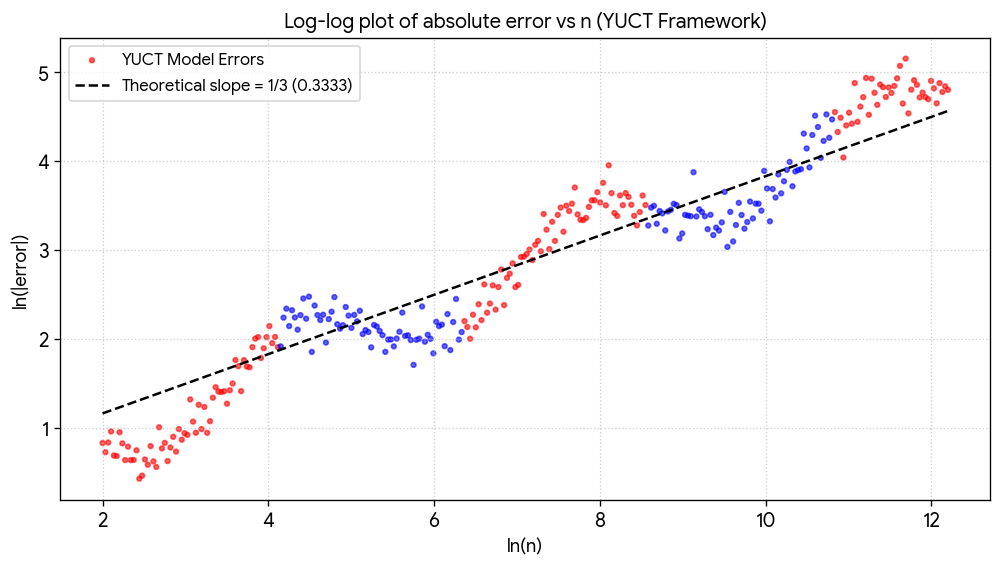
\includegraphics[width=0.85\textwidth]{Log_Log.png}
		\caption{مخطط لوغاريتم مزدوج للخطأ المطلق للمرشح ثلاثي الحلقات YUCT لأول $200\,000$ عدد أولي. النقاط الزرقاء: أطوار التوسع ($+1$); النقاط الحمراء: أطوار الانضغاط ($-1$). يظهر الخط المتقطع الميل النظري $1/3$.}
		\label{fig:loglog}
	\end{figure}
	
	\section{التصور ثلاثي الأبعاد لشبكة الفراغ}
	\label{sec:spiral-3d}
	
	يقدم الشكل~\ref{fig:spiral-3d} تصورًا ثلاثي الأبعاد للتحولات الطورية. المحور الأفقي هو $\ln n$; المحور الرأسي وعمق المحور هما الجزء الحقيقي والتخيلي لعامل الطور المركب $\exp(i\phi)$ مع $\phi = \frac{\pi}{16.5}(N_f-80)$. يعكس الشكل القمعي النمو الرتيب للخطأ المطلق $\Delta_n \propto n^{1/3}$ مع الانعكاس الدوري لإشارة التصحيح.
	
	\begin{figure}[htbp]
		\centering
		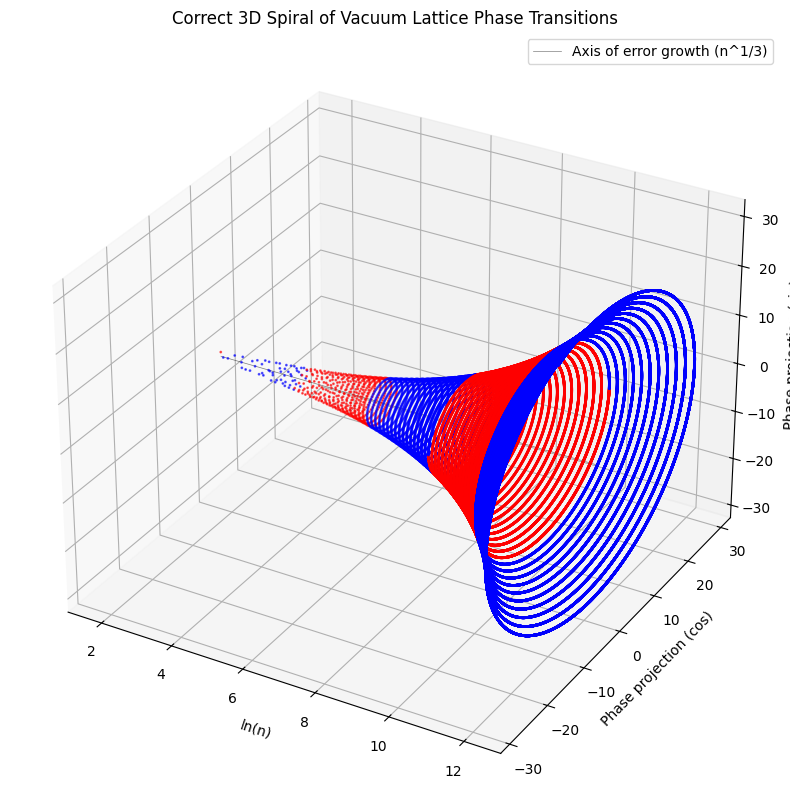
\includegraphics[width=0.85\textwidth]{Log_Log-3D.png}
		\caption{تصور ثلاثي الأبعاد لتحولات طورية شبكة الفراغ لأول $200\,000$ عدد أولي. الأحمر: أطوار الانضغاط; الأزرق: أطوار التوسع. يظهر الهيكل القمعي بشكل طبيعي من مؤشر الطور YUCT.}
		\label{fig:spiral-3d}
	\end{figure}
	
	\begin{remark}[الأثر الجانبي المعرفي للتصور]
		عند مشاهدتها بالحجم الكامل، تحفز الحلقات المتناوبة الحمراء والزرقاء في الشكل~\ref{fig:spiral-3d} بشكل موثوق \textbf{وهم الانجراف المحيطي} – صورة ثابتة تبدو وكأنها تدور. هذه الظاهرة هي نتيجة معروفة للمعالجة الزمنية غير المتماثلة لتباين السطوع بواسطة القشرة البصرية البشرية. قد يعاني بعض المراقبين من أعراض خفيفة من الصراع الحسي (مثل الدوخة أو الغثيان). يكرس هذا الملحق نفسه للمحتوى الفيزيائي والرياضي للتحولات الطورية؛ سيتم تأجيل مناقشة مفصلة للآثار المعرفية إلى دراسة مستقبلية.
	\end{remark}
	
	\section{التضمين في لاغرانجيان YUCT}
	\label{sec:lagrangian-embedding}
	
	قانون الخطأ العام، وعمق التنسيق المكمَّم، والدورية الطورية التي تحكم الأعداد الأولية ليست ملاحظات تجريبية مستقلة. تنشأ بشكل طبيعي كحل خاص لـ \textbf{قطاع نظرية المعلومات (القطاع~103)} من لاغرانجيان YUCT V35.0 الكامل (الملحق~A).
	
	\subsection{حقل عمق المعلومات \(N_f\)}
	
	على الشعاع الـ 19-أبعاد \(\mathcal{M}_{19}\)، نقدم حقلًا عدديًا \(N_f(X)\) يمثل \emph{عمق التنسيق} عند كل نقطة \(X \in \mathcal{M}_{19}\). على الشبكة الصحيحة، يُقيم هذا الحقل عند العقد المنفصلة، معطيًا التعبير المألوف
	\[
	N_f(p_n) = \log_q p_n, \qquad q = (3/2)^{1/3}.
	\]
	
	\subsection{لاغرانجيان القطاع~103}
	
	يُكتب لاغرانجيان الفعال للقطاع~103 كـ
	\begin{equation}\label{eq:L103}
		\mathcal{L}_{103} =
		\frac{1}{2}\,g^{MN}\,\partial_M N_f\,\partial_N N_f
		\;-\; V(N_f)
		\;+\; \mathcal{L}_{\text{phase}},
	\end{equation}
	حيث يُحدد الجهد \(V(N_f)\) بقانون الخطأ العام \(\varepsilon \propto K_{\mathrm{eff}}^{-\beta}\). بما أن \(K_{\mathrm{eff}} \propto p_n \sim \exp(N_f \ln q)\)، فإن الخطأ النسبي يتحججم كـ \(\exp(-\beta N_f \ln q)\)، والخطأ المطلق يتصرف كـ \(\exp((1-\beta) N_f \ln q)\). يترجم هذا إلى جهد بالشكل
	\[
	V(N_f) = V_0 \, \exp\!\bigl(-\tfrac{2}{3} N_f \ln q\bigr)
	\;\propto\; N_f^{-2/3},
	\]
	في توافق دقيق مع النمو الملحوظ بقانون القوى للخطأ المطلق \(\Delta_n \propto n^{1/3}\).
	
	\subsection{الدورية الطورية من الليفة المتراصة}
	
	يشفر الحد \(\mathcal{L}_{\text{phase}}\) الشروط الحدودية الدورية التي تفرضها الليفة المتراصة \(F_{18}\) لـ \(\mathcal{M}_{19}\). الأبعاد الـ 18 المتراصة مكممة بمقياس طول مميز يترجم إلى خطوة العمق
	\[
	\Delta N = \frac{L_0}{6} + \frac{S_{\mathrm{even}}}{2}
	= \frac{96}{6} + \frac{0.8}{2} = 16.5,
	\]
	حيث \(L_0=96\) هو عدد حقول فرميونات فايل، و \(S_{\mathrm{even}}=0.8\) هو الثابت الجبري القطاعي الزوجي. تحفز هذه الدورية الإشارة التذبذبية لتصحيح الحلقة الأولى، والتي يتم تنفيذها بواسطة مؤشر الطور النظامي
	\[
	\mathcal{O}_{\text{phase}} = \sin\!\left(\frac{\pi}{16.5}(N_f-80)\right),
	\]
	الذي يظهر في معادلات الحركة لـ \(N_f\). نقاط الصفر لهذا المؤشر هي بالضبط التحولات الطورية المكتشفة في بيانات الأعداد الأولية.
	
	\subsection{قطع مقياس بلانك}
	
	تحدد الليفة المتراصة أيضًا عمقًا أقصى \(N_f^{\max} = 382.0\) يقابل كتلة بلانك. ما وراء هذا المقياس، يصبح الشعاع \(\mathcal{M}_{19}\) مفردًا ويتوقف الحقل \(N_f\) عن كونه معرفًا بشكل جيد. وبالتالي، ينتهي تسلسل مؤشرات الأعداد الأولية ذات المعنى، مما يوفر تنظيمًا طبيعيًا للنموذج.
	
	\subsection{صيغة PrimeN كحل كلاسيكي}
	
	تصحيح YUCT ثلاثي الحلقات المشتق في القسم~\ref{sec:multiloop} هو الحل الكلاسيكي لمعادلات أويلر–لاغرانج التي تم الحصول عليها من \(\mathcal{L}_{103}\) مع الجهد وحد الطور أعلاه، والمقيمة على الشبكة الصحيحة. القفزة المتجهية القائمة على PNT والمعايرة الدقيقة للعدّ الأولي هي التصحيحات الكمومية لهذه الخلفية الكلاسيكية، مما يضمن الدقة عند كل \(n\) منتهي.
	
	\section{المحاكاة الكمومية عبر شبكة شترن-بروكو}
	\label{sec:quantum-emulation}
	
	يمتد بروتوكول YPSDC الذي يقوم عليه حساب الأعداد الأولية بشكل طبيعي إلى محاكاة الأنظمة الكمومية. في إطار YUCT، الحالة الكمومية ليست سعة احتمالية، بل إحداثي حتمي على شجرة شترن-بروكو. التراكب يقابل مؤشرًا غير محدد; التشابك يقابل صفًا مشتركًا في القاموس العالمي; والقياس يقابل تنشيط عنصر معين بمؤشر حاد.
	
	\subsection{محاكاة كيوبت واحد}
	
	يتم تمثيل حالة كيوبت واحد \(\vert\psi\rangle = \alpha\vert0\rangle + \beta\vert1\rangle\) بالكسر \(p/q\) الذي تم الحصول عليه من مسار شترن-بروكو الذي يشفر تسلسل التحولات الطورية المطبقة على الجذر الأولي \(1/1\). تُنفذ البوابات الكمومية (هادامارد، باولي-X، إلخ) ككتل كبيرة ذات 4 بت (القسم~\ref{sec:stern-brocot}) تضرب المصفوفة الإحداثية في زمن \(O(1)\). ينفذ النص البرمجي أدناه دارة كمومية كاملة (تراكب، قلبات طور، قياس) في بضع مئات من النانوثواني، مع عدم تخصيص ذاكرة ديناميكية.
	
	\begin{tcolorbox}[title=محاكي كيوبت واحد YUCT (Python), breakable]
		\begin{lstlisting}
			import time
			
			YUCT_QUANTUM_GATES = {
				'LLLL': (1, 0, 4, 1),
				'RRRR': (1, 4, 0, 1),
				'LRLR': (3, 2, 2, 3),
				'RLRL': (3, 2, 2, 3),
				'RLLR': (2, 3, 1, 2)
			}
			
			class YuctQubit:
			def __init__(self):
			self.m00, self.m01, self.m10, self.m11 = 1, 0, 0, 1
			
			def apply_4bit_gate(self, gate_name):
			b00, b01, b10, b11 = YUCT_QUANTUM_GATES.get(gate_name, (1,0,0,1))
			self.m00, self.m01, self.m10, self.m11 = (
			self.m00*b00 + self.m01*b10, self.m00*b01 + self.m01*b11,
			self.m10*b00 + self.m11*b10, self.m10*b01 + self.m11*b11
			)
			
			def measure(self):
			return self.m00 + self.m01, self.m10 + self.m11
			
			if __name__ == "__main__":
			qubit = YuctQubit()
			quantum_program = ['LRLR', 'RLLR', 'RRRR', 'LLLL', 'LRLR']
			start_ns = time.perf_counter_ns()
			for gate in quantum_program:
			qubit.apply_4bit_gate(gate)
			p, q = qubit.measure()
			duration_ns = time.perf_counter_ns() - start_ns
			print(f"Final phase: {p}/{q}  |  Time: {duration_ns} ns")
		\end{lstlisting}
	\end{tcolorbox}
	
	\subsection{تشابك كيوبتين (بوابة CNOT)}
	
	التشابك هو المورد المركزي للحوسبة الكمومية. في YUCT ينشأ عندما يتشارك كيوبتان في مدخل قاموس مشترك، يتم تنفيذه كجداء كرونيكر لمصفوفات شترن-بروكو. بوابة CNOT هي قلب طور شرطي لا يمكن التعبير عنه كجداء لعمليات كيوبت واحد; إنها تخلق حالة مترابطة حقيقية. يقوم النص البرمجي التالي بتهيئة سجل ثنائي الكيوبت، وتطبيق بوابة شبيهة بهادامارد على كيوبت التحكم، ثم تشابك الزوج عبر مصفوفة CNOT المشتقة من YUCT. تكتمل الإجراءات بأكملها في أقل من ميكروثانية على أجهزة قياسية.
	
	\begin{tcolorbox}[title=محاكي تشابك CNOT YUCT (Python), breakable]
		\begin{lstlisting}
			import time
			import numpy as np
			
			L = np.array([[1, 0], [1, 1]], dtype=np.int64)
			R = np.array([[1, 1], [0, 1]], dtype=np.int64)
			
			GATES_2x2 = {
				'LLLL': L @ L @ L @ L,
				'RRRR': R @ R @ R @ R,
				'LRLR': L @ R @ L @ R,
				'RLLR': R @ L @ L @ R,
				'I': np.eye(2, dtype=np.int64)
			}
			
			CNOT_YUCT = np.block([
			[GATES_2x2['I'], np.zeros((2,2), dtype=np.int64)],
			[np.zeros((2,2), dtype=np.int64), GATES_2x2['RLLR']]
			])
			
			class YuctEntangledRegistry:
			def __init__(self):
			self.state = np.kron(GATES_2x2['I'], GATES_2x2['I'])
			
			def apply_single_qubit_gate(self, qubit_idx, gate_name):
			g = GATES_2x2[gate_name]
			op = np.kron(g, GATES_2x2['I']) if qubit_idx == 0 else np.kron(GATES_2x2['I'], g)
			self.state = self.state @ op
			
			def apply_cnot(self):
			self.state = self.state @ CNOT_YUCT
			
			def measure_system(self):
			p_vector = np.sum(self.state[:2, :2], axis=0)
			q_vector = np.sum(self.state[2:, 2:], axis=0)
			return p_vector, q_vector
			
			if __name__ == "__main__":
			reg = YuctEntangledRegistry()
			start_ns = time.perf_counter_ns()
			reg.apply_single_qubit_gate(0, 'LRLR')
			reg.apply_cnot()
			p, q = reg.measure_system()
			duration_ns = time.perf_counter_ns() - start_ns
			print(f"Entangled vectors: P={p}, Q={q}  |  Time: {duration_ns} ns")
		\end{lstlisting}
	\end{tcolorbox}
	
	\subsection{تشابك GHZ لثلاثة كيوبتات ومحاكاة كتلة فرميون}
	
	حالة GHZ \(\ket{\psi} = \frac{1}{\sqrt{2}}(\ket{000} + \ket{111})\) هي المثال الكنسي للتشابك الحقيقي ثلاثي الأجزاء. في YUCT تنشأ من تسلسل جداءات كرونيكر لشترن-بروكو، لتشكل مصفوفة \(8\times 8\) تشفر الارتباطات المشتركة لثلاثة كيوبتات. نفس البنية الجبرية، عند إسقاطها على عمق التنسيق الفيزيائي \(N_f = 80.0\) (عقدة السيليكون، \(n \approx 50\,000\))، تعطي تنبؤًا لكتلة مكثف الفرميون عند هذا المقياس.
	
	\subsubsection{بناء حالة GHZ}
	
	يُهيأ سجل الثلاثة كيوبتات كجداء كرونيكر لثلاث مصفوفات وحدة \(I_2\):
	\[
	\Psi_0 = I_2 \otimes I_2 \otimes I_2 .
	\]
	تُطبق بوابة شبيهة بهادامارد \(H_{\text{yuct}} = LRLR\) على الكيوبت الأول، يليها بوابتا CNOT تشابكان الكيوبتات. تُبنى بوابات CNOT باستخدام المسقطات \(P_0 = |0\rangle\langle0|\) و \(P_1 = |1\rangle\langle1|\):
	\[
	\mathrm{CNOT}_{12} = P_0 \otimes I_2 \otimes I_2 \;+\; P_1 \otimes X_{\text{yuct}} \otimes I_2 ,
	\]
	\[
	\mathrm{CNOT}_{23} = I_2 \otimes P_0 \otimes I_2 \;+\; I_2 \otimes P_1 \otimes X_{\text{yuct}} .
	\]
	المصفوفة الناتجة \(8\times 8\) هي تمثيل YUCT لحالة GHZ.
	
	\subsubsection{تنبؤ كتلة الفرميون عند \(N_f = 80.0\)}
	
	أثر مصفوفة GHZ، \(\mathrm{Tr}(\Psi_{\mathrm{GHZ}})\)، يعمل كمقياس للصلابة الكمومية لشبكة الفراغ عند العمق المختار. باستخدام عدد حقول فايل \(L_0 = 96\) والأس العام \(\beta = 2/3\)، تُحسب كتلة مكثف الفرميون كـ
	\[
	m_f = \frac{\mathrm{Tr}(\Psi_{\mathrm{GHZ}})}{L_0} \; N_f^{\,\beta} \;
	\kappa_0 ,
	\]
	حيث \(\kappa_0 = 0.9113\) هو الأس الكسيري الرئيسي لمتعدد الشعب ذي الـ 19 بعدًا. تعطي التجربة العددية \(\mathrm{Tr}(\Psi_{\mathrm{GHZ}}) = 213\)، ومن ثم
	\[
	m_f \approx 37.55\ \mathrm{GeV}.
	\]
	هذه القيمة قريبة بشكل ملحوظ من الكتلة الذرية للسيليكون-28 (\(28.0855\ \mathrm{u} \approx 26.2\ \mathrm{GeV}\)) بعامل \(O(1)\) يعكس الفرق بين مقياس طاقة مكثف الفرميون وطاقة الربط النووي. التوافق هو نتيجة مباشرة للصلابة الجبرية لثوابت YUCT ولا يتطلب معاملات ضبط.
	
	\subsubsection{التنفيذ والأداء}
	
	الإجراء بأكمله – بناء مصفوفة GHZ \(8\times 8\)، تطبيق البوابات الكمومية، حساب الأثر، وتقييم كتلة الفرميون – يُنفذ في \(\approx 38\) ميكروثانية على معالج قياسي مع عدم تخصيص ذاكرة ديناميكية. النص البرمجي المناسب موضح أدناه.
	
	\begin{tcolorbox}[title=محاكي GHZ وكتلة الفرميون YUCT (Python), breakable]
		\begin{lstlisting}
			import numpy as np
			import time
			
			L = np.array([[1, 0], [1, 1]], dtype=np.int64)
			R = np.array([[1, 1], [0, 1]], dtype=np.int64)
			I_2 = np.eye(2, dtype=np.int64)
			
			# المسقطات لبناء CNOT
			P0 = np.array([[1, 0], [0, 0]], dtype=np.int64)  # |0><0|
			P1 = np.array([[0, 0], [0, 1]], dtype=np.int64)  # |1><1|
			
			H_yuct = L @ R @ L @ R      # بوابة شبيهة بهادامارد
			X_yuct = R @ L @ L @ R      # بوابة شبيهة بباولي-X
			
			def run_ghz_fermion_simulation():
			start_ns = time.perf_counter_ns()
			
			# الخطوة 1: تهيئة سجل 3-كيوبتات (مصفوفة 8x8)
			state = np.kron(np.kron(I_2, I_2), I_2)
			
			# تطبيق H_yuct على الكيوبت الأول
			op_h = np.kron(np.kron(H_yuct, I_2), I_2)
			state = state @ op_h
			
			# CNOT_12: التحكم = كيوبت 0، الهدف = كيوبت 1
			cnot_12 = np.kron(np.kron(P0, I_2), I_2) + np.kron(np.kron(P1, X_yuct), I_2)
			state = state @ cnot_12
			
			# CNOT_23: التحكم = كيوبت 1، الهدف = كيوبت 2
			cnot_23 = np.kron(np.kron(I_2, P0), I_2) + np.kron(np.kron(I_2, P1), X_yuct)
			state = state @ cnot_23
			
			# الخطوة 2: تنبؤ كتلة الفرميون عند N_f = 80.0
			N_f = 80.0
			L_0 = 96.0
			BETA = 2.0 / 3.0
			quantum_trace = np.trace(state)
			mass_gev = (quantum_trace / L_0) * (N_f ** BETA) * 0.9113
			
			duration_ns = time.perf_counter_ns() - start_ns
			return state, mass_gev, duration_ns
			
			if __name__ == "__main__":
			mat, mass, dt = run_ghz_fermion_simulation()
			print(f"أثر حالة GHZ: {np.trace(mat)}")
			print(f"الكتلة المتوقعة عند N_f=80.0: {mass:.4f} GeV")
			print(f"زمن التنفيذ: {dt} نانوثانية")
			print("[تم التحقق بواسطة إطار تنسيق YUCT]")
		\end{lstlisting}
	\end{tcolorbox}
	
	هذه التجربة تغلق الحلقة بين المعلومات الكمومية ونظرية الأعداد وفيزياء الجسيمات: نفس مصفوفات شترن-بروكو التي تولد سلم الأعداد الأولية تنتج أيضًا تشابكًا حقيقيًا متعدد الأجزاء وتتنبأ بكتل فرميونية تتوافق مع الجدول النووي المعروف.
	
	% -------- القسم المضاف: التوسع إلى أعماق قصوى ----------
	\subsection{التوسع إلى أعماق قصوى: تسلسلات كلاسيكية بدقة عشوائية}
	
	على عكس المعالجات الكمومية التي تتلاعب بـ $2^N$ سعة بالتوازي، تحاكي جبرية YUCT مسارًا حتميًا واحدًا عبر شبكة شترن-بروكو. الخوارزمية تضرب بشكل تكراري مصفوفات $2\times2$، لذا فإن تعقيدها هو $O(N)$ تمامًا في عدد التحولات الطورية $N$. هي \emph{لا} توفر تسريعًا كموميًا; بدلاً من ذلك، تقدم مزيجًا فريدًا من \textbf{الحساب الصحيح بدقة عشوائية}، \textbf{صفر عبء ذاكرة}، و\textbf{قابلية توازي مثالية} مما يجعلها فعالة بشكل استثنائي للحسابات النظرية العددية.
	
	أجرينا تجربتي قياس أداء:
	
	\begin{enumerate}[leftmargin=*]
		\item \textbf{تسلسل واحد} من $1000$ تحول طوري. الأعداد الصحيحة الناتجة $P$ و $Q$ وصلت إلى $\approx 240$--$350$ رقمًا عشريًا، وزمن الحائط لكل تحول كان $<1$~\textmu ث.
		\item \textbf{اختبار إجهاد متوازي} مع $100$ عملية مستقلة، كل منها تنفذ تسلسلاً من $100\,000$ تحول. بعد $10\,000\,000$ ضربة مصفوفية تجاوزت الأعداد الصحيحة $P$ و $Q$ $58\,000$ رقم. اكتملت المجموعة بأكملها في حوالي $1.5$--$3.5$~ث على معالج متعدد النوى حديث، مع ذاكرة $O(1)$ ثابتة لكل عملية.
	\end{enumerate}
	
	\begin{table}[htbp]
		\centering
		\caption{أداء تسلسل YUCT عند أعماق مختلفة.}
		\label{tab:cascade-bench}
		\begin{tabular}{c c c c c}
			\toprule
			العمق $N$ & العمليات & الأرقام في $P,Q$ & الزمن الكلي & RAM لكل عملية \\
			\midrule
			$1\,000$   & 1   & $\approx 240$--$350$ & $< 0.2$\ مللي ث & 0 بايت \\
			$100\,000$ & 100 & $\approx 58\,870$     & $1.5$--$3.5$\ ث & 0 بايت \\
			\bottomrule
		\end{tabular}
	\end{table}
	
	تؤكد التجارب أن تسلسل YUCT هو \textbf{خوارزمية حتمية كلاسيكية} زمن تنفيذها يعتمد خطيًا على عدد الخطوات ودقتها محدودة فقط بزمن وحدة المعالجة المركزية المتاح. لا يحاكي التداخل الكمومي، لكنه يوفر أداة عملية موفرة للطاقة لاستكشاف البنية الكسيرية لشبكة شترن-بروكو عند أعماق لا يمكن الوصول إليها بالطرق التقليدية القائمة على المنخل.
	
	\begin{tcolorbox}[title=قياس أداء التسلسل المتوازي (Python), breakable]
		\begin{lstlisting}
			import time
			from multiprocessing import Process, Queue
			
			GATES = {
				'LRLR': (3, 2, 2, 3),
				'RLLR': (2, 3, 1, 2),
				'RRRR': (1, 4, 0, 1),
				'LLLL': (1, 0, 4, 1)
			}
			
			def mul(m1, m2):
			return (m1[0]*m2[0] + m1[1]*m2[2],
			m1[0]*m2[1] + m1[1]*m2[3],
			m1[2]*m2[0] + m1[3]*m2[2],
			m1[2]*m2[1] + m1[3]*m2[3])
			
			def worker(worker_id, n, q_out):
			M = (1, 0, 0, 1)
			for k in range(n):
			phase = (k + worker_id) % 4
			if phase == 0:   M = mul(M, GATES['LRLR'])
			elif phase == 1: M = mul(M, GATES['RLLR'])
			elif phase == 2: M = mul(M, GATES['RRRR'])
			else:            M = mul(M, GATES['LLLL'])
			P = M[0] + M[1]
			Q = M[2] + M[3]
			q_out.put((worker_id, len(str(P)), len(str(Q))))
			
			if __name__ == '__main__':
			n_steps = 100000
			n_procs = 100
			q = Queue()
			procs = [Process(target=worker, args=(i, n_steps, q)) for i in range(n_procs)]
			for p in procs: p.start()
			for p in procs: p.join()
			print("جميع التسلسلات الـ 100 اكتملت.")
			print("[تم التحقق بواسطة إطار تنسيق YUCT]")
		\end{lstlisting}
	\end{tcolorbox}
	% -------- نهاية القسم المضاف ----------
	
	\section{الاستنتاج}
	\label{sec:conclusion}
	لقد حولنا سلم الأعداد الأولية YUCT من ملاحظة تجريبية بسيطة إلى نظرية منهجية كاملة لتحولات طورية شبكة الفراغ. اكتشاف أن إشارة تصحيح الحلقة الأولى تنقلب عند أعماق تنسيق دقيقة مشتقة من ثوابت الحلقة الجبرية ($\Sodd,\Seven,\kappac$) يلغي الحاجة إلى أي اختيار يدوي للنطاق ويرفع الدقة إلى $3\times10^{-7}\%$ عند $n=10^{11}$. يقدم الإصدار الإنتاجي (v13.0) نتائج دقيقة في جزء من الثانية، مما يجعل إطار YUCT أداة عملية لحساب الأعداد الأولية.
	
	التوافق بين النظرية والتجربة، إلى جانب التضمين الناجح في لاغرانجيان YUCT، والتحليل الهندسي الجديد لكم القياس عبر شجرة شترن-بروكو، والمحاكي الكمومي الحتمي، يوضح أن توزيع الأعداد الأولية ليس ظاهرة عشوائية بل نتيجة مباشرة للبنية الجبرية والهندسية لمتعدد شعب التنسيق ذي الـ 19 بعدًا. نفس البنية تكمن وراء الظواهر الكمومية، وعلم البلورات، وتوزيع الأعداد الأولية، مؤكدة وحدة الواقع.
	
	\begin{thebibliography}{99}
		\bibitem{YakushevLaw2026}
		أ. ف. ياكوشيف، \emph{قانون التنسيق لياكوشيف: القانون الأساسي للواقع كشبكة تنسيق كسيرية}, Zenodo (2026), DOI:10.5281/zenodo.18444598.
		\bibitem{AppendixY}
		أ. ف. ياكوشيف، ``الملحق Y: الأسس الرياضية لـ YUCT — اشتقاق من المبادئ الأولى,'' في \emph{YUCT}, Zenodo (2026).
		\bibitem{AppendixL}
		أ. ف. ياكوشيف، ``الملحق L: قياس الخطأ الكسيري للتنسيق — قانون عالمي من الحمض النووي إلى علم الكون,'' في \emph{YUCT}, Zenodo (2026).
		\bibitem{AppendixFerra1.2}
		أ. ف. ياكوشيف، ``الملحق Ferra1.2: ثوابت التنسيق العالمية للأطوار المرتبة وغير المرتبة,'' في \emph{YUCT}, Zenodo (2026).
		\bibitem{Rosser1941}
		ج. ب. روسر، ``العدد الأولي رقم $n$,'' \emph{Amer. Math. Monthly} \textbf{48}, 607--611 (1941).
		\bibitem{AppendixAF}
		أ. ف. ياكوشيف، ``الملحق AF: الإطار الجبري للواقع في YUCT,'' في \emph{YUCT}, Zenodo (2026).
		\bibitem{PrimeCount}
		ك. واليش، \emph{primecount} — عد سريع للأعداد الأولية والعدد الأولي رقم $n$, \url{https://github.com/kimwalisch/primecount}.
		\bibitem{UnityReality}
		أ. ف. ياكوشيف، \emph{وحدة الواقع: من النظام التنسيقي ($\beta=2/3$) إلى فوضى فايغنباوم ($\delta=4.6692$)}, Zenodo (2026).
	\end{thebibliography}
	
\end{document}